% Indicate the main file. Must go at the beginning of the file.
% !TEX root = ../main.tex

%%%%%%%%%%%%%%%%%%%%%%%%%%%%%%%%%%%%%%%%%%%%%%%%%%%%%%%%%%%%%%%%%%%%%%%%%%%%%%%%
% 06_declaration
%%%%%%%%%%%%%%%%%%%%%%%%%%%%%%%%%%%%%%%%%%%%%%%%%%%%%%%%%%%%%%%%%%%%%%%%%%%%%%%%


\section{Declaration}
\label{declaration}

\subsection{Declaration of AI Usage}%%%%%%%%%%%%%%%%%%%%%%%%%%%%%%%%%%%%%%%%%%%%%%

\textbf{GitHub Copilot} was active during all coding tasks as well as text writing in this thesis.
While it was primarily intended to assist with LaTeX formatting, it also provided suggestions for the text itself.
For the actual coding tasks, it was used to help solve problems, generate code snippets and played a significant role in debugging.

\textbf{ChatGPT Model o4-mini} was used to assist with coding, problem-solving and debugging.
\textbf{ChatGPT GPT-4o} and \textbf{GPT-4.5} were used to support content research, thesis structuring, writing and refining the text.
The Abstract was initially generated and translated using \textbf{ChatGPT GPT-4o}.
Both versions where thoroughly reviewed and manually edited.
Every paragraph was finally fed into \textbf{GPT-4o} for a final spelling and grammar check --- all changes were manually reviewed using a git diff viewer to ensure that no unwanted edits were introduced.

\newpage
\refstepcounter{subsection}
\addcontentsline{toc}{subsection}{\protect\numberline{\thesubsection}Statement of Authorship}

\newgeometry{left=0in, right=0in, top=0.5in, bottom=0in}
\thispagestyle{empty}
\begin{figure}[h!]
    \centering
    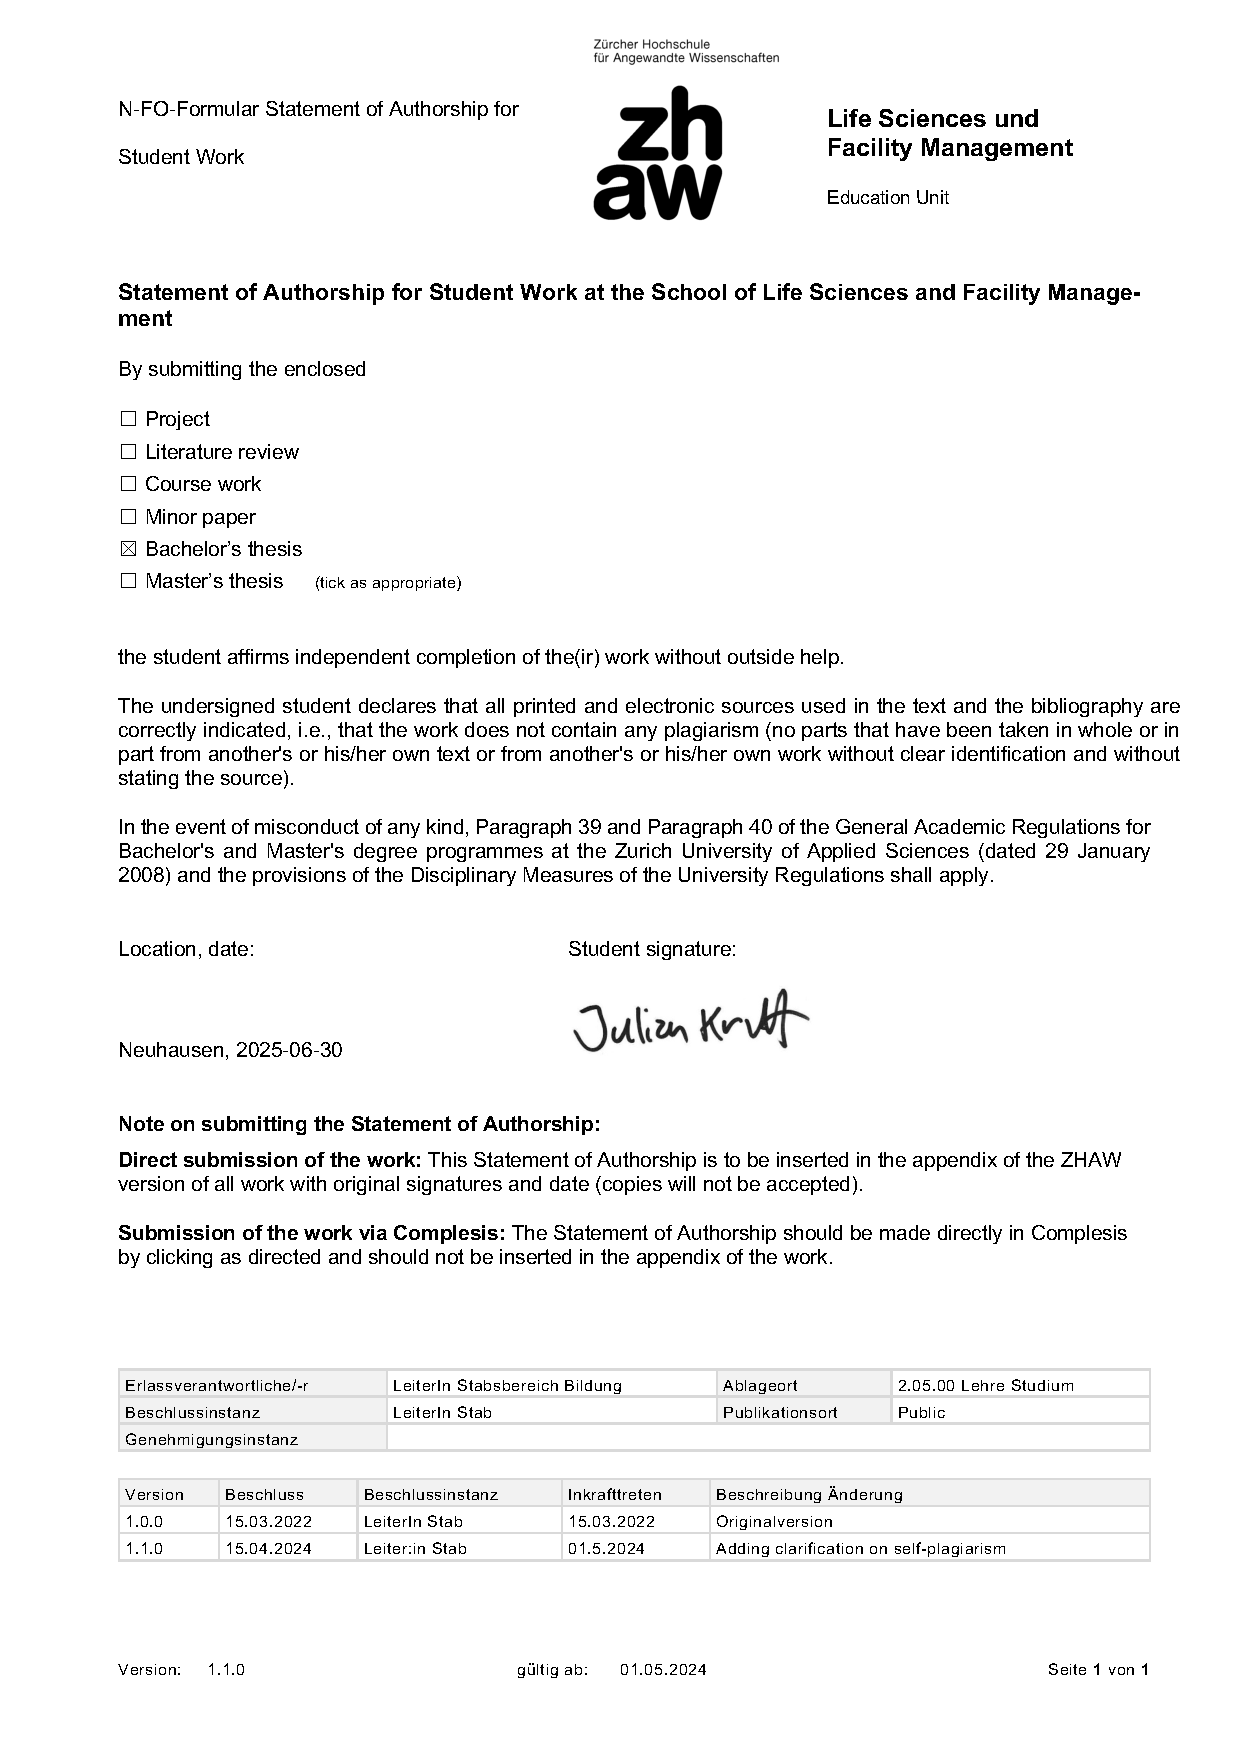
\includegraphics[width=0.9\textwidth]{appendix/declaration_independence.pdf}
\end{figure}
\restoregeometry % Restore original margins
